The edge device processing pipeline presented in Figure \ref{fig:edges} illustrates a compact and efficient architecture designed specifically for CPU-based edge devices equipped with a single-core CPU operating at 3.5 GHz and limited memory capacity of 512 MB RAM. This streamlined approach optimally addresses the constraints of computational resources while performing real-time video analytics directly at the network edge.

\begin{figure}[htbp]
    \centering
    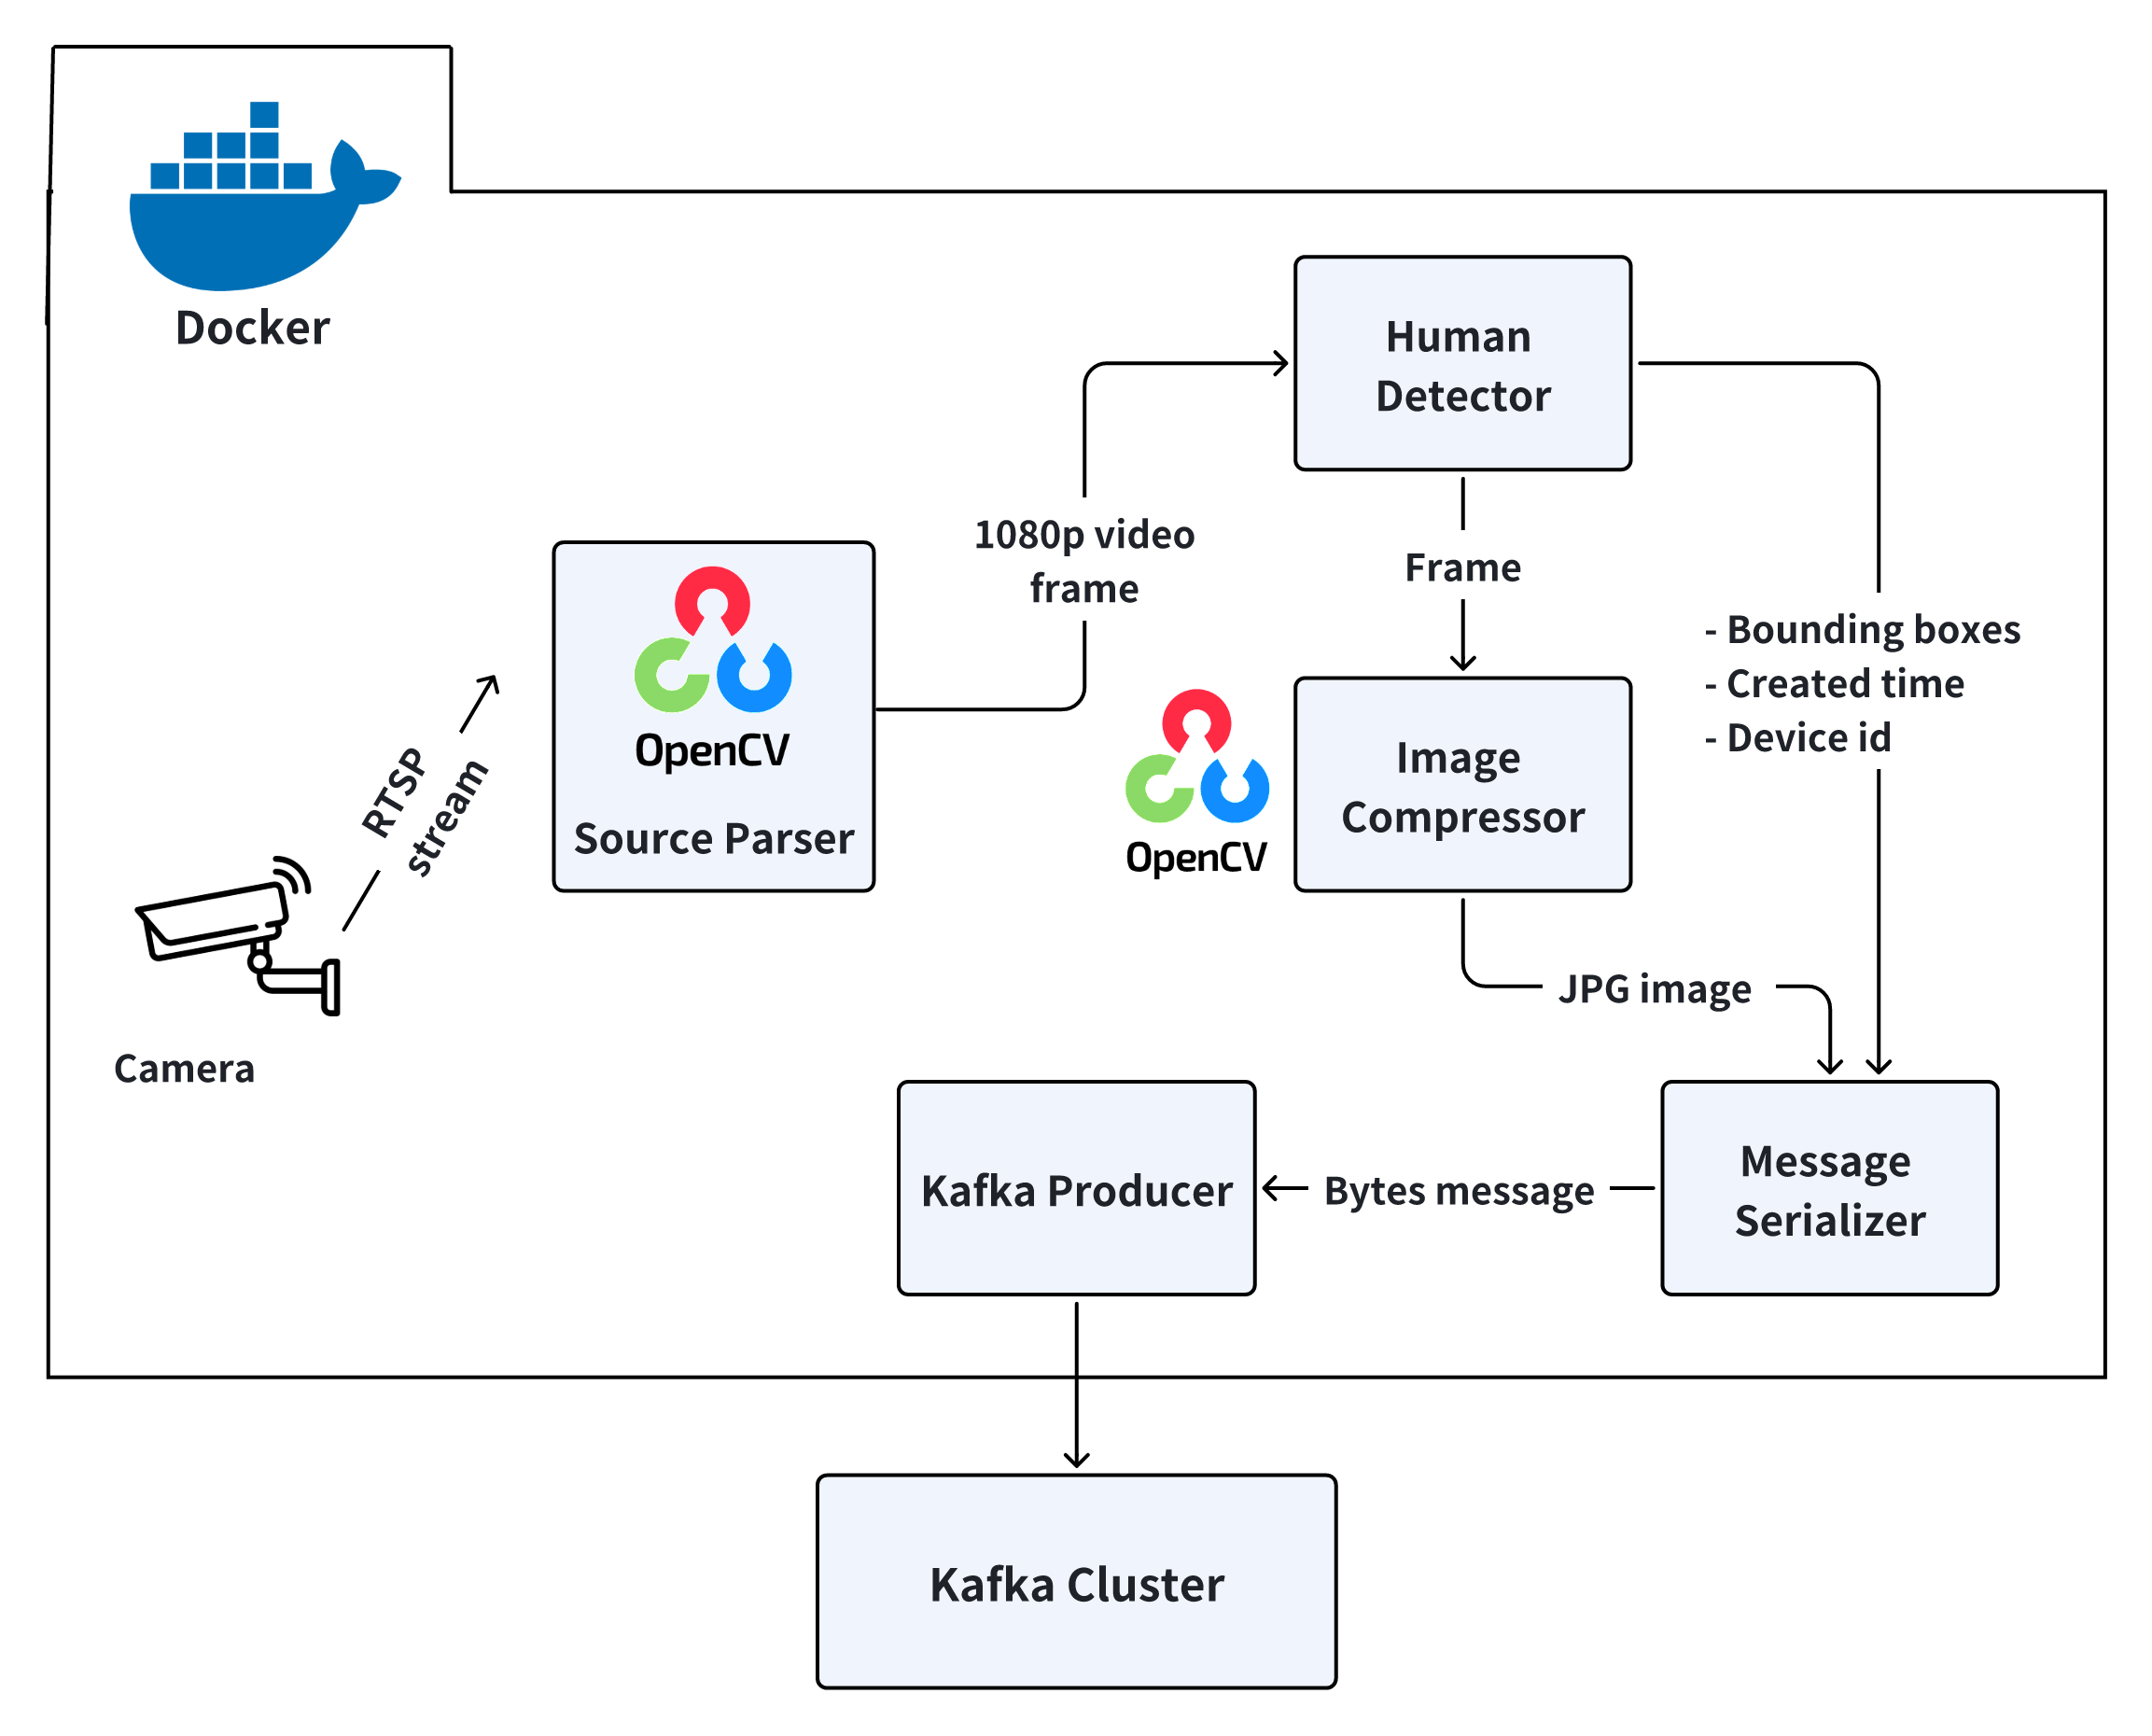
\includegraphics[width=1\textwidth]{Figure/edges.png}
    \caption{Edge devices processing pipeline}
    \label{fig:edges}
\end{figure}

The pipeline operates through several integrated components that work together to achieve efficient video processing:

\begin{itemize}
    \item \textbf{Source parser}: This component handles input from RTSP cameras delivering live video streams and stored H264 video sources. Both inputs are uniformly processed through an OpenCV-based source parser that standardizes the video streams into 1080p frames, thus simplifying subsequent processing steps and minimizing resource overhead.
    
    \item \textbf{Detection model}: The standardized video frames are then processed by a lightweight yet robust YOLOv11 object detection model, excellently suited for human detection. This detection module identifies human subjects within each frame, generating precise bounding box coordinates and essential metadata such as timestamp and device identifier.
    
    \item \textbf{Image Compressor}: To further optimize resource usage, the original video frames undergo simultaneous compression using OpenCV's image processing capabilities, producing compressed JPG images. This significantly reduces the data size, essential for constrained CPU environments, without compromising analytical quality.
    
    \item \textbf{Message Serializer}: Detection results along with the compressed images are efficiently structured into Avro schema serialized messages, significantly improving serialization speed and resource efficiency.
    
    \item \textbf{Kafka producer}: Finally, these structured messages are published to Kafka topics through a dedicated lightweight producer, enabling seamless real-time communication with cloud-based analytics platforms and further downstream processing systems.
\end{itemize}

This targeted approach ensures minimal resource consumption, reduced network bandwidth requirements, prompt local analytics responses, and increased scalability by distributing the analytical load across multiple constrained edge devices.

The following sections provide detailed implementation descriptions for each component, beginning with the \textbf{Human detection with YOLOv11} module.

\subsection{Human detection with YOLOv11}
\label{sec:edge_human_detection}

\subsection{Image compression with OpenCV}
\label{sec:edge_image_compression}

\subsection{Messages serialization with Avro schema}
\label{sec:edge_message_serialization}

\subsection{Produce messages to Kafka}
\label{sec:edge_produce_messages}

\subsection{Containerization with Docker}
\label{sec:edge_containerization}